\ifx\boi\undefined\ifx\problemname\undefined
\providecommand\sampleinputname{}
\providecommand\sampleoutputname{}
\documentclass[norsk]{templates/boi}
\problemlanguage{.no}
\fi
\newcommand{\boi}{Baltic Olympiad in Informatics}
\newcommand{\practicesession}{Practice Session}
\newcommand{\contestdates}{April 27 - May 1, 2018}
\newcommand{\dayone}{Dag 1}
\newcommand{\daytwo}{Dag 2}
\newcommand{\licensingtext}{This problem is licensed under CC BY-SA 4.0.}
\newcommand{\problem}{Problem}
\newcommand{\inputsection}{Input}
\newcommand{\outputsection}{Output}
\newcommand{\interactivity}{Interaktivitet}
\newcommand{\grading}{Grading}
\newcommand{\scoring}{Scoring}
\newcommand{\constraints}{Begrensninger}
\renewcommand{\sampleinputname}{Sample Input}
\renewcommand{\sampleoutputname}{Sample Output}
\newcommand{\sampleexplanation}[1]{Forklaring av eksempel #1}
\newcommand{\sampleexplanations}{Eksempelforklaring}
\newcommand{\timelimit}{Time Limit}
\newcommand{\memorylimit}{Memory Limit}
\newcommand{\seconds}{s}
\newcommand{\megabytes}{MB}
\newcommand{\group}{Group}
\newcommand{\points}{Points}
\newcommand{\limitsname}{Limits}
\newcommand{\additionalconstraints}{Yttligere begrensninger}
\newcommand{\testgroups}{
Løsningen din vil bli testet på et sett av testgrupper, hver verdt et visst antall poeng.
Hver testgruppe inneholder et sett av tester.
For å få poeng for en testgruppe må du løse alle testene i den gruppen.
Din endelige poengsum vil være den høyeste poengsummen du har fått på en enkelt innlevering.
}
\fi
\def\version{jury-1}
\problemname{Vekselstrøm}
Fredrik leker med en model-jernbane som han har bygd selv og er veldig stolt av.
Jernbanen består av $N$ segmenter sem er koblet i en sirkel, nummerert $1, 2, \dots, N$ i klokkeretning.
Toget får strøm gjennom $M$ kontaktledninger som går langs jernbanen. Hvert segment har minst én ledning som går langs den.

Fredrik er litt lei av at toget konstant går rundt og rundt og har bestemt seg for å legge til \emph{sporveksler} på hvert segment, som han kan bruke til å lage avsporinger og andre artigheter.
Men disse vekslene trenger også strøm. Og ikke bare hva slags strøm som helst -- siden de er veksler så trenger de selvfølgelig \emph{vekselstrøm}.

Fredrik er ikke helt sikker, men han tror at måten man får vekselstrøm på er ved å ha strøm som går i begge retninger. Hver
ledning gir bare strøm i én retning (enten med klokka, eller mot klokka) men Fredrik kan fritt velge hvilken.
Det vil si at han ønsker å gjøre et valg om retningen av strømmen i hver ledning, slik at hvert sporsegment får strøm
både fra en ledning hvor strømmen går i klokkeretning og en ledning hvor strømmen hvor strømmen går mot klokkeretning.

Kan du hjelpe Fredrik med dette?

\vspace{2mm}
%\hspace*{2mm}
\begin{center}
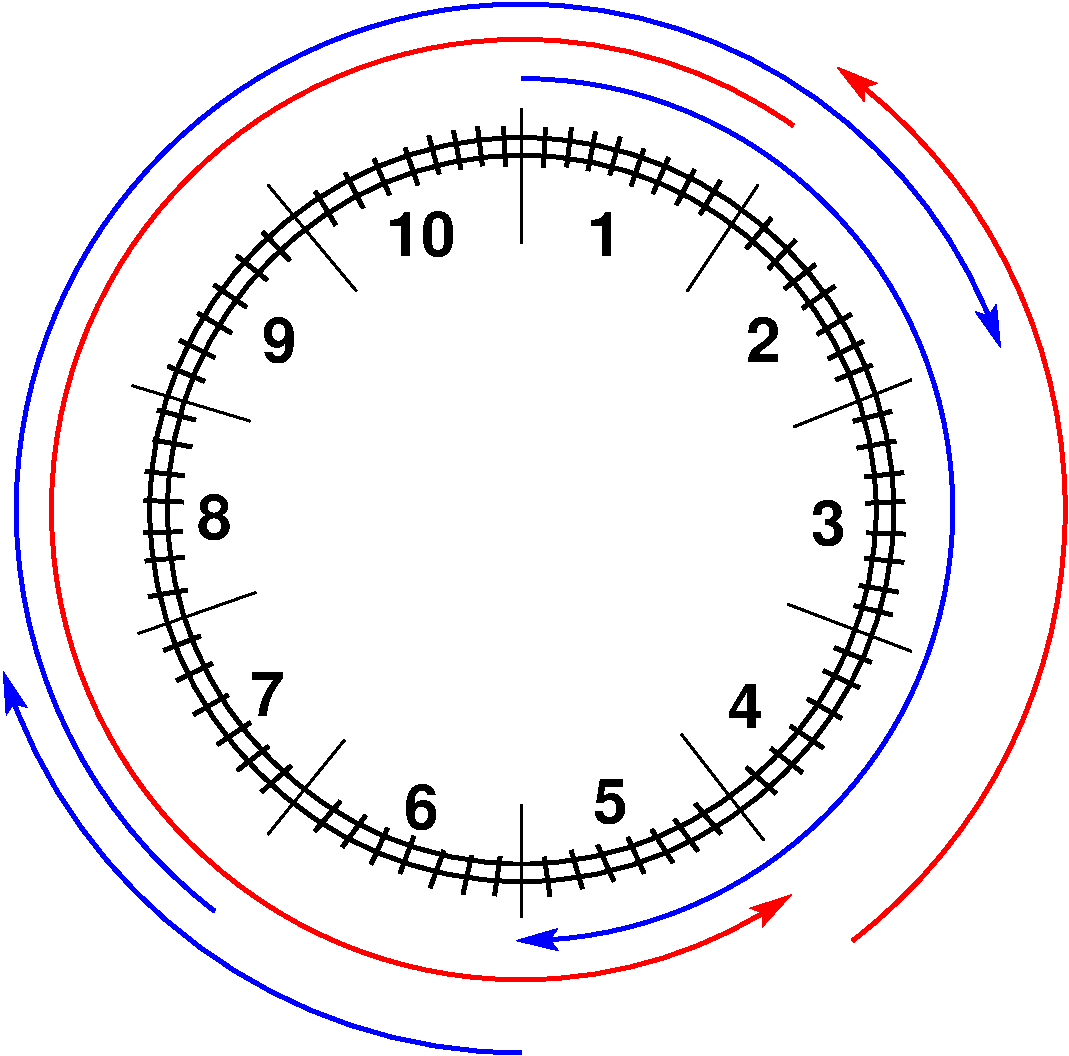
\includegraphics[width=0.5\textwidth]{alternatingfig.pdf}
\end{center}
\vspace{1mm}
{\em En løsning til første input. De buede pilene utenfor jernbanen representerer ledningene som gir strøm.
Retningen av hver pil representerer Fredriks valg av retning på strømmen (de er også farget blåe og røde for
å illustrere retningene). Merk at alle pilene kunne ha blitt snudd for å gi den andre gyldige løsningen: \texttt{11010}.}

\section*{\inputsection}
Første linje inneholder to heltall $N$ og $M$, henholdsvis antall jernbanesegmenter og antall ledninger.

De neste $M$ linjene inneholder hver to tall $1 \le a, b \le N$, som indikerer at det er en ledning
som dekker segmentene $a, a+1, \dots, b$. Dersom $b$ er mindre enn $a$ så betyr det at sekvensen \emph{går rundt},
altså at den dekker segmentene $a, \dots, N, 1, \dots, b$. Merk at hvis $a=b$, så dekker ledningen kun det ene segmentet.

\section*{\outputsection}
Skriv ut en enkelt linje med $M$ tegn, hvor hvert tegn er enten \texttt{0} eller \texttt{1}.
Det $i$-te tegnet på linjen skal være \texttt{0} hvis strømmen i den $i$-te ledningen gitt i input skal gå i klokkeretning,
eller \texttt{1} hvis strømmen skal gå mot klokka.
Hvis det finnes flere løsninger kan du skrive ut hvilken som helst av de.

Hvis det ikke er noen gyldig løsning skal du skrive ut ``\texttt{impossible}''.

\section*{\constraints}
\testgroups

\noindent
\begin{tabular}{| l | l | l | l |}
\hline
\textbf{\group} & \textbf{\points} & \textbf{\limitsname} & \textbf{\additionalconstraints} \\ \hline
  1     & 13     & $2 \le N, M \le 15$ & \\ \hline
  2     & 20     & $2 \le N, M \le 100$ & \\ \hline
  3     & 22     & $2 \le N, M \le 1000$ & \\ \hline
  4     & 19     & $2 \le N, M \le 100\,000$ & Ingen ledning har $b < a$. \\ \hline
  5     & 26     & $2 \le N, M \le 100\,000$ & \\ \hline
\end{tabular}

